\documentclass[conference]{IEEEtran}
%\IEEEoverridecommandlockouts
% The preceding line is only needed to identify funding in the first footnote. If that is unneeded, please comment it out.
\usepackage{cite}
\usepackage{amsmath,amssymb,amsfonts}
\usepackage{algorithmic}
\usepackage{graphicx}
\usepackage{textcomp}
\usepackage{xcolor}
% \usepackage[
% backend=biber,
% style=alphabetic,
% sorting=ynt
% ]{biblatex}
% \addbibresource{biblio.bib}
% \def\BibTeX{{\rm B\kern-.05em{\sc i\kern-.025em b}\kern-.08em
%     T\kern-.1667em\lower.7ex\hbox{E}\kern-.125emX}}

\title{Progress Report}

\begin{document}


\author{\IEEEauthorblockN{1\textsuperscript{st} Mykhailo Dmytrenko}
    \and
    \IEEEauthorblockN{2\textsuperscript{nd} Antonio Sgorbissa}

}

\maketitle
\section{Introduction}
In this brief overview the current progress of the project will be discussed, highlighting different
points of interest, as well as plans for the future work.In the context of human SLAM for environmental disasters, there are currently several subjects of the main focus : \textbf{Karto - SLAM}, \textbf{Onthologies}, \textbf{Voice recognition} and usage of \textbf{extra sensors - Thingy91}, \textbf{Deterministic loop closure} and \textbf{Microsoft HoloLens map visualization}.



\section{Karto - SLAM}
Following the work of the Master thesis student who worked on this project, Karto-SLAM was
chosen as a framework for the graph-based SLAM. The above-mentioned was improved significantly
perfomance-wise and was able to successfully generate a graph based map real-time with a size of
120 by 55.6 meters with 2706 nodes in total with 1 forced loop closure and 7 automatic closures. The result can be seen in Fig. \ref{map}.
\begin{figure}[htbp]
    \centerline{\includegraphics[width=0.5\textwidth,height=\textheight,keepaspectratio]{Pictures/rviz_screenshot_2021_03_22-16_01_59.png}}
    \caption{Optimized Map built in real-time}

    \label{map}

\end{figure}

\section{Ontology}



A major introduction to the loop closure algorithm are ontologies.
The words were chosen according to the typical landmarks which are typically seen in the urban environment - in this case the historical centre of Genova. Example photo can be seen in Fig.\ref{street view}. Corresponding ontology tree is depicted on the Fig.\ref{onto}.

Several Python scripts automatically read and generate lists of words compatible
with the speech recognition engine as well as with graph-based SLAM.

\begin{figure}[htbp]
    \centerline{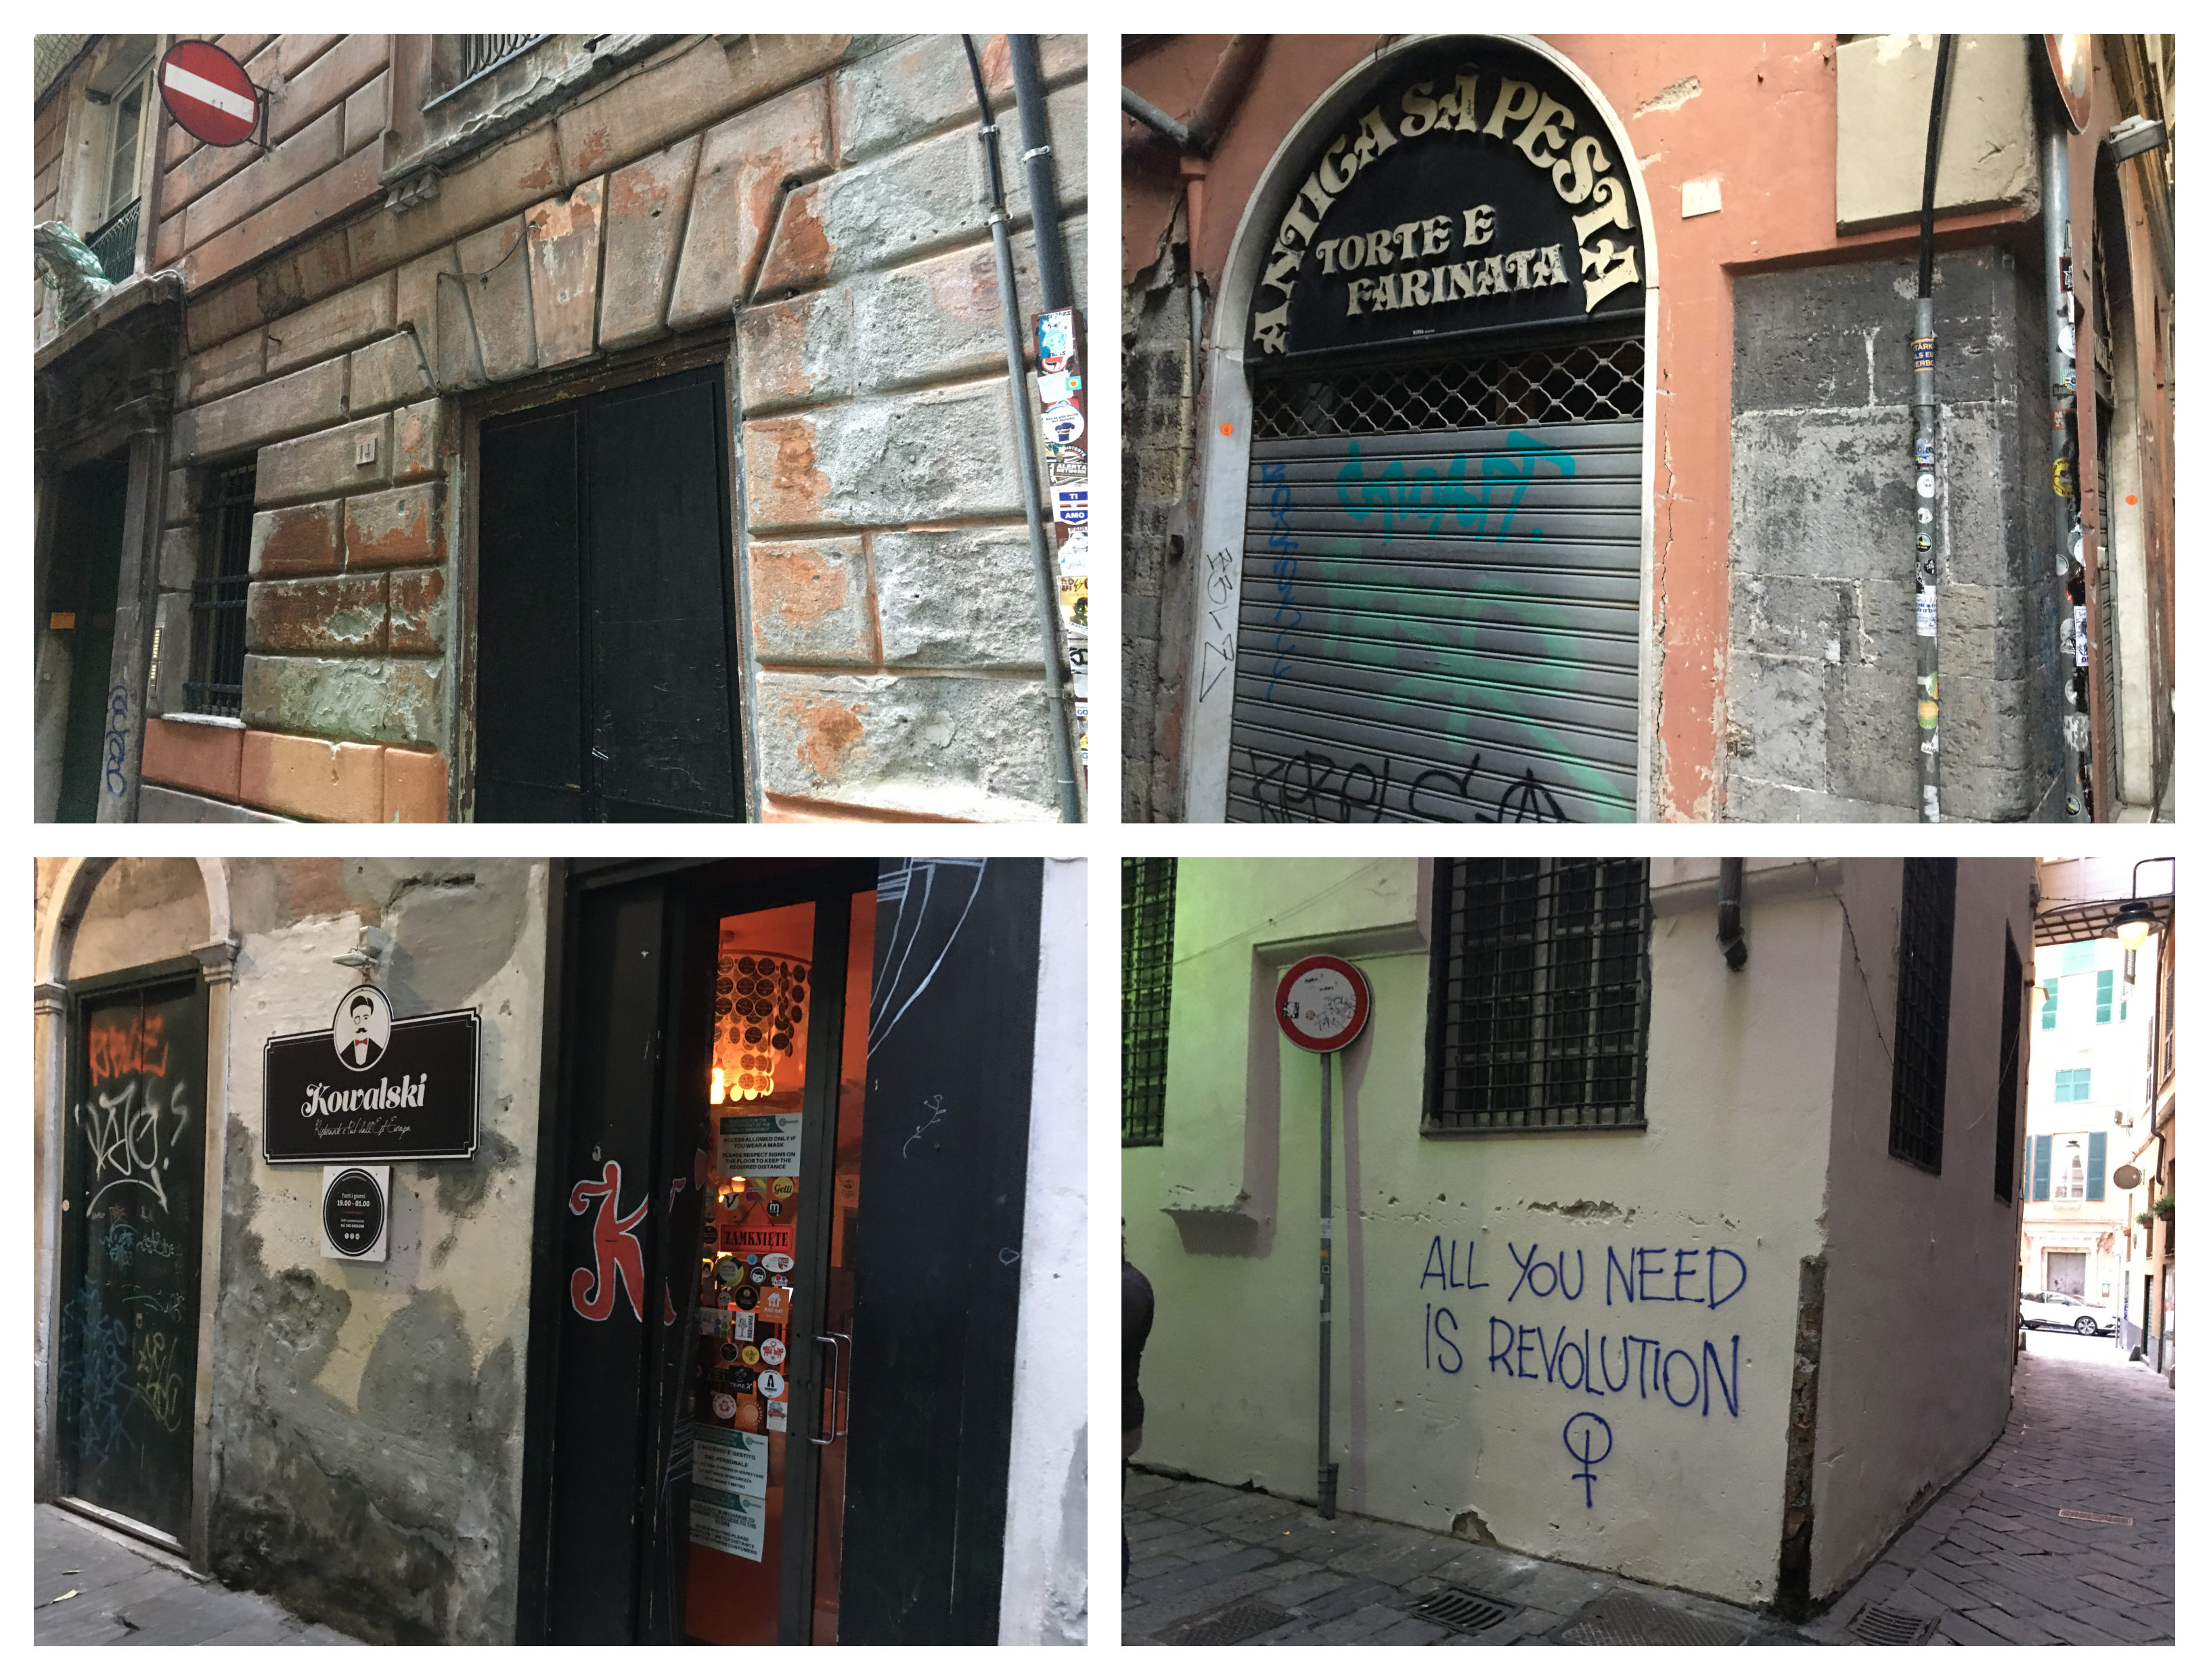
\includegraphics[width=0.5\textwidth,height=\textheight,keepaspectratio]{Pictures/05.jpg}}
    \caption{Example photo of the streetview}

    \label{street view}

\end{figure}



\begin{figure}[htbp]
    \centerline{\includegraphics[width=0.5\textwidth,height=0.4\textheight,keepaspectratio]{Pictures/onto.png}}
    \caption{Ontology generated}

    \label{onto}
\end{figure}



\section{Voice recognition - Picovoice}

Finding a reliable ofline recognition engine presented a major challenge. Initially,
CMU Sphinx recognizer \cite{sphinx} has been chosen. However, it failed to prove to be usable enough for the needed application. The main issues were unrecognizable words, false negatives and inability to recognize all words in the ontology at once. A different engine was chosen called \textbf{Picovoice} \cite{pico}. It is an efficient offline solution which uses compressed neural networks and can work on resource-restrained microcontrollers. It was successfully adapted to the current application in tandem with the ontology and it is able to recognize all 94 words of current ontology at once. 

There are two main tecnologies included in Picovoice - \textbf{Porcupine} \cite{porcupine} wake word engine and \textbf{Rhino} \cite{rhino} Speech-to-Intent Engine. Porcupine proved to be a very accurate wake word engine. It contains a list of pre-trained words, which can be used for the activation of the listening process. In addition to this, there is a possibility to train custom words using Picovoice console. Once the wake word is detected, Rhino engine gets activated. After a list of words to detect has been added, it is possible to train and download the model. Afterwards, the two models (from Porcupine and Rhino engines) can be used in a Python scripts on the local machine, hence once all models are downloaded the speech recognition process can work completely offline.

\section{Extra sensors}

In the context of environmental disasters there is also a need to gather extra information about the environment - temperature, vibrations, humidity etc. Thingy91 from Nordic Semiconductor \cite{thingy} is a battery operated prototyping system with a multitude of sensors for motion, impact, air quality and much more. In addition to this, Nordic Semiconductors offers a cloud which gets all the data from the kit through the cellular data connection which than can be retrieved from anywhere. The kit supports NB-IoT and LTE-M, which are both communication technologies for IoT devices which work with cellular data. In Italy only NB-IoT is supported. 


\begin{figure}[htbp]
    \centerline{\includegraphics[width=0.5\textwidth,height=0.2\textheight,keepaspectratio]{Pictures/NRF6943.jpg}}
    \caption{Thingy91 development platform}

    \label{thingy_pic}
\end{figure}

The readily available data is visualized on the \textbf{nrfCloud}, which is seen on Fig. \ref{nrfCloud_pic}. This data can accessed as a JSON file with a curl command for further processing in Python script.

\begin{figure}[htbp]
    \centerline{\includegraphics[width=0.5\textwidth,height=0.2\textheight,keepaspectratio]{Pictures/nrfCloud.png}}
    \caption{nrfCloud data visualization}

    \label{nrfCloud_pic}
\end{figure}

The main issue with this develiopment kit is that detailed accelerometer data is not available in the current software version. Instead, it is in the under developing section and is currently explored.

\section{Software overview}

The general overview of the ROS nodes can be seen on Fig.\ref{ROS}.For the audio input \textbf{Mapper} is listening for the word index which is then added to the graph node as a custom object. Then, in order to make use of semantic distances these indices are converted back into words where the ontologies information can be used again through a ROS service \textbf{dist$\_$service}.

\section{Deterministic loop closure}

Currently, deterministic loop closure algorithm uses 3 parameters to decide how to close the loop: laser scan response, physical distance and semantic distance. Each special node gets compared with the newly-added one. 
In case several criteria are met, the edge strength is determined proportionally to the above-mentioned parameters. E.g. the covarience of the link created is smaller the closer the nodes are to each other.

\begin{figure}[htbp]
    \centerline{\includegraphics[width=0.5\textwidth,height=\textheight,keepaspectratio]{Pictures/overview_ROS.png}}
    \caption{Overview of ROS structure}

    \label{ROS}

\end{figure}

\section{Microsoft Hololens Map Visualization}

There are some ready made tools available to save the map to the server in order to be visualized with Microsoft Hololens. One example is \textbf{map$\_$server} in ROS, however it saves only the map without any frames or extra information, which can be a problem in the future. Instead it would be much more beneficial to save the entire RVIZ view, which can be done with \textbf{rviz$\_$camera$\_$stream}. This approach requires much more customization but more beneficial in the long run. \cite{rhino}







\bibliographystyle{IEEEtran}
\typeout{}
\bibliography{biblio}





\end{document}